\documentclass{estilo}
\usepackage[spanish]{babel}
\usepackage{graphicx}
\usepackage{float}
\usepackage{amsmath}        % para los vectores columnas
\usepackage{amsfonts}       % para las negrita de pizarra
\usepackage{amssymb}        % para simbolos matematicos
\usepackage{hyperref}       % para utilizar referencias
\usepackage{multirow}       % para las tablas
\usepackage{dsfont}
\usepackage{listings}
\usepackage{xcolor}
\definecolor{codegreen}{rgb}{0,0.6,0}
\definecolor{codegray}{rgb}{0.5,0.5,0.5}
\definecolor{codepurple}{rgb}{0.58,0,0.82}
\definecolor{backcolour}{rgb}{0.95,0.95,0.92}
\lstdefinestyle{mystyle}{
    backgroundcolor=\color{backcolour},   
    commentstyle=\color{codegreen},
    keywordstyle=\color{magenta},
    numberstyle=\tiny\color{codegray},
    stringstyle=\color{codepurple},
    basicstyle=\ttfamily\footnotesize,
    breakatwhitespace=false,         
    breaklines=true,                 
    captionpos=b,                    
    keepspaces=true,                 
    numbers=left,                    
    numbersep=5pt,                  
    showspaces=false,                
    showstringspaces=false,
    showtabs=false,                  
    tabsize=2
}
\lstset{style=mystyle}

\usepackage{enumitem,multicol,setspace}
\newcounter{subenum}[enumi] % para las multicolumnas
\renewcommand{\thesubenum}{\arabic{subenum}}
\usepackage[nomessages]{fp}
\FPeval\thecolwidth{round(1/4:4)}% Specify number of columns -> column width
\newcommand{\newitem}[1]{%
  \refstepcounter{subenum}%
  \parbox{\dimexpr\thecolwidth\linewidth-.5\columnsep}{%
    \makebox[\labelwidth][r]{(\thesubenum)\hspace*{\labelsep}}%
    #1}\hfill%
}

\usepackage{scalerel,stackengine} % para el sombrero
\stackMath
\newcommand\rhat[1]{%
\savestack{\tmpbox}{\stretchto{%
  \scaleto{%
    \scalerel*[\widthof{\ensuremath{#1}}]{\kern-.6pt\bigwedge\kern-.6pt}%
    {\rule[-\textheight/2]{1ex}{\textheight}}%WIDTH-LIMITED BIG WEDGE
  }{\textheight}% 
}{0.5ex}}%
\stackon[1pt]{#1}{\tmpbox}%
}
\parskip 1ex

\usepackage{mathtools}      % floor y ceil
\DeclarePairedDelimiter\ceil{\lceil}{\rceil}
\DeclarePairedDelimiter\floor{\lfloor}{\rfloor} 

\usepackage[style=authoryear-comp]{biblatex}


\begin{document}
\maketitle

\justifying{}

\newpage
\section{Consideraciones}

Este documento está pensado para que sirva de guía, e incluso template a la hora de realizar un informe para la materia (por no decir, cualquier documento formal en la facultad). La idea es utilizar \LaTeX, pura y exclusivamente para que tenga un formato acorde. Es decir, no hecho en un simple procesador de texto (como pudiese ser Word). 

Aquí sólo se mostraran algunas de las cosas que se pueden hacer con \LaTeX. Si se quiere hacer algo específico, o de otra forma, abunda la documentación (y artículos de StackOverflow) al respecto. 

Definimos ciertos lineamientos técnicos a considerar para los informes: 
\begin{itemize}
    \item En el informe debe estar incluido el código más importante (es decir, los algoritmos, no un main) cuando corresponda. 
    \item Debe estar explicado cómo se hacen los sets de prueba. Inclusive, si notan alguna falencia con esta generación que pueda afectar de alguna forma el análisis del resultado, se espera que lo enuncien (hay trabajos donde esto no sucederá, pero hay trabajos donde sí, especialmente cuando vemos aproximaciones). 
    \item Los gráficos deben estar bien generados: deben tener título, los ejes deben tener tanto qué refieren como qué unidad de medida usan (en caso de tenerla). En caso de tener gráficos superpuestos, debe quedar claro qué es cada gráfico. 
    \item \textbf{Importante}: en caso de tener que realizar una reentrega (y por ende, tener que cambiar cosas del informe), salvo que haya que rehacer una enorme cantidad del mismo, no modificar el informe anterior sino agregar un anexo al final indicando las correcciones realizadas en la nueva entrega, para agilizar las correcciones. 
\end{itemize}

A su vez, dejamos algunas breves líneas sobre cuestiones de redacción: 
\begin{itemize}
    \item Evitar errores ortográficos y gramaticales. 
    \item El lenguaje debe ser técnico. No tiene que por eso ser un texto aburrido, pero evitar frases como "\textit{la cosa que más me complicó fue...}", "\textit{creo que...}". 
    \item Usar plural de modestia, incluso si el trabajo fuera realizado por una única persona.
\end{itemize}
\newpage
\justifying{
\hypertarget{res}{\section*{Ejemplo de Resolución}}
\section{Algoritmo para encontrar el máximo}

En este trabajo de ejemplo realizaremos el análisis teórico y empírico de diferentes algoritmos que sirven para resolver el mismo problema: obtener el valor del máximo elemento de un arreglo desordenado de $n$ elementos. 

\subsection{Algoritmo Iterativo}

A continuación se muestra el código de solución iterativa del problema. 

\begin{lstlisting}[language=Python]
def maximo(datos):
    max_pos = 0
    for i in range(1, len(datos)):
        if datos[i] > datos[max_pos]:
            max_pos = i
    return datos[max_pos]
\end{lstlisting}

% Si queremos importar el código directo desde un archivo, podemos hacer lo siguiente: 

% \lstinputlisting[language=Python]{code/maximo_iterativo.py}

% Ventaja: evitamos copiar y pegar, y que si en un momento se modifique el algoritmo (reentrega, o la razón que fuere) no nos tengamos que acordar de esto más allá de compilar. 

% Desventaja: tenemos que asegurarnos de modularizar el código en archivos en función de cómo queremos mostrar el informe. Por otro lado, esto tiene especial sentido si estamos trabajando todo de forma local. Es decir, en el caso que no usemos Overleaf, porque sino implica tener que copiar el código de todas formas. 

% Mencionamos esta alternativa para que sepan que existe, ustedes definen cómo prefieren trabajar con esto. No nos interesa el código del informe, sólo el pdf resultante. 

La complejidad del algoritmo propuesto para encontrar el máximo es $\mathcal{O}(n)$, debido a que para cada elemento del arreglo se realizan operaciones $\mathcal{O}(1)$.


\subsection{Algoritmo por División y Conquista}

A continuación, mostramos la implementación de un algoritmo que encuentra el máximo de un arreglo por División y Conquista. Es decir, busca el máximo que corresponde al subarreglo izquierdo, lo mismo para el derecho y se queda con el máximo entre ambos \textit{sub máximos}.

\begin{lstlisting}[language=Python]
def maximo(datos):
    if len(datos) == 1:
        return 0    
    
    izq = maximo(datos[:len(datos)//2])
    der = maximo(datos[len(datos)//2:])
    return izq if izq > der else der
\end{lstlisting}

La ecuación de recurrencia que corresponde a este algoritmo es: 
\begin{equation*} %nota: el asterisco es para que no aparezca el (1) al lado de la ecuación
    \mathcal{T}(n) = 2 \mathcal{T}\left(\frac{n}{2}\right) + \mathcal{O}(n)
\end{equation*}

Esto es porque tenemos 2 llamados recursivos, cada lado con la mitad del problema, y al partir hacemos una slice, lo cual en Python realiza una copia, por lo cual demora tiempo lineal en aplicarse en cada caso. 

Aplicando el teorema maestro, la complejidad nos queda en $\mathcal{O}\left(n \log n\right)$. En este caso, nos quedó peor complejidad que en el caso iterativo pura y exclusivamente por abusar del lenguaje de programación sin tomar en cuenta el tiempo que consume hacer un slice. Dejando de hacer esto, podemos mostrar la siguiente versión del algoritmo: 

\begin{lstlisting}[language=Python]
def maximo(datos):
    return maximo_dyc(datos, 0, len(datos) - 1)

def maximo_dyc(datos, inicio, fin):
    if inicio == fin:
        return datos[inicio]

    medio = (inicio + fin) / 2
    izq = maximo_dyc(datos, inicio, medio)
    der = maximo_dyc(datos, medio + 1, fin)
    return izq if izq > der else der
\end{lstlisting}

En este caso, la ecuación de recurrencia es: 
\begin{equation*}
    \mathcal{T}(n) = 2 \mathcal{T}\left(\frac{n}{2}\right) + \mathcal{O}(1)
\end{equation*}

Aplicando el teorema maestro, nos queda que la complejidad es $\mathcal{O}\left(n\right)$.

Es importante notar que en otros lenguajes de programación esto podría no ser necesario (por ejemplo, Go). En algunos lenguajes se puede operar usando Slices que consuman $\mathcal{O}(1)$ de tiempo (a cambio de utilizar la misma memoria que el arreglo original), o bien usando aritmética de punteros como puede ser el caso de C. Independientemente del caso, es importante notar que el algoritmo de división y conquista es lógicamente igual (o extremadamente similar), pero tenemos que considerar cuestiones de implementación del lenguaje elegido a la hora de definir las complejidades. 

\section{Mediciones}

Se realizaron medicions en base a crear arreglos de diferentes largos, yendo de 100 en 100 elementos, donde los elementos en cada caso fueron generados por los valores pseudoaleatorios del lenguaje (el módulo \texttt{random}). 

\begin{figure}[H]
    \centering
    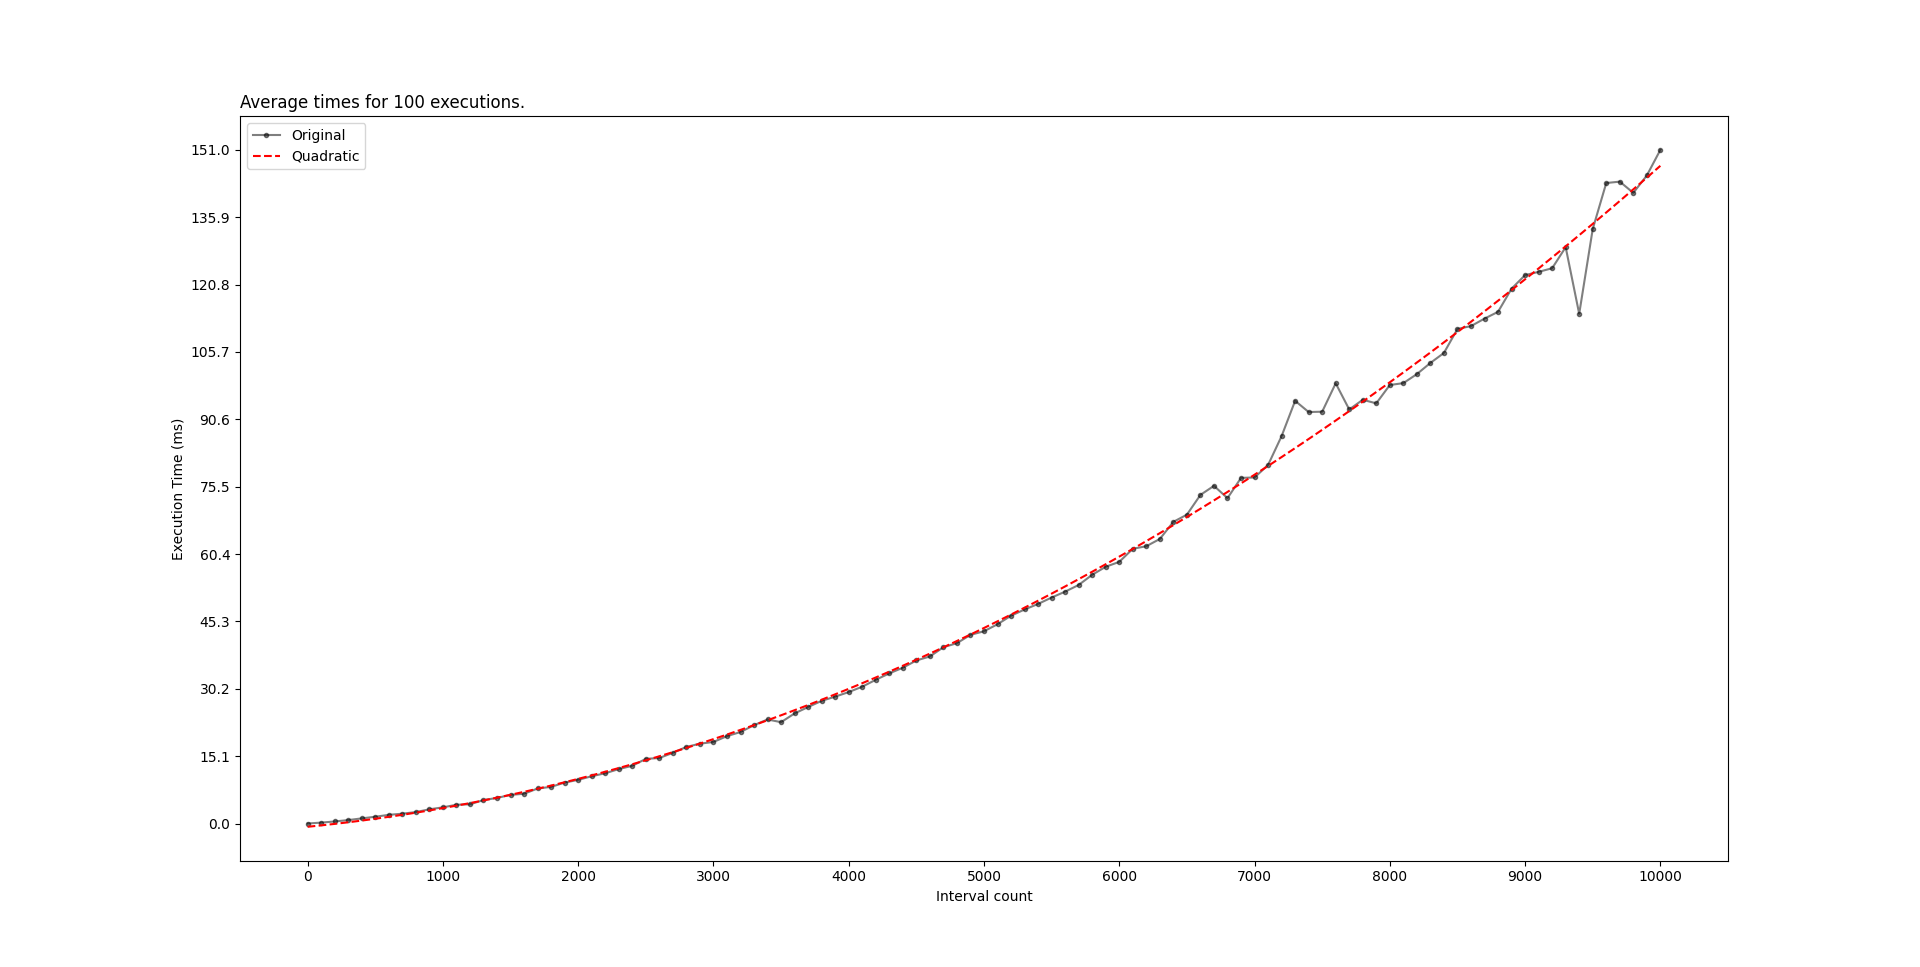
\includegraphics[width=1\textwidth]{../images/graphic_100Intervals.png}
    Este gráfico muestra el tiempo de ejecución promedio de 100 ejecuciones del programa (en milisegundos) dada una cantidad de intervalos con un acomodo cuadrático
\end{figure}

\begin{figure}[H]
	\centering
	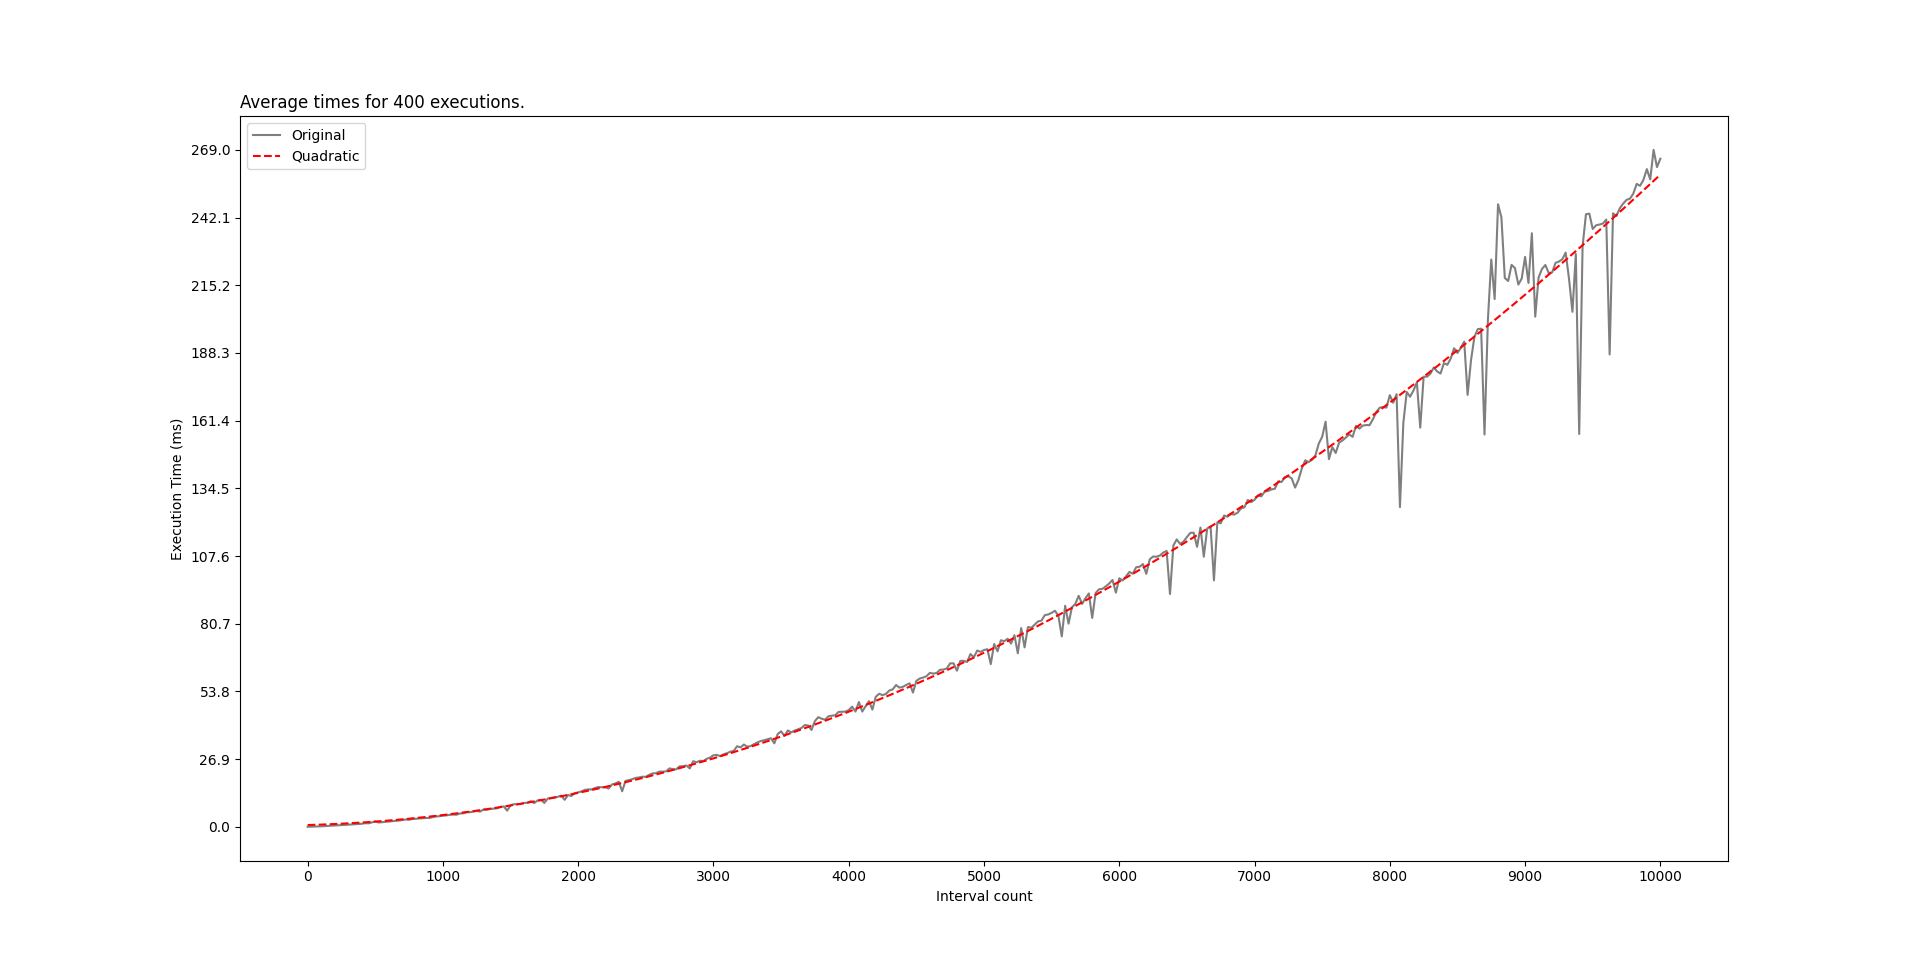
\includegraphics[width=1\textwidth]{../images/graphic_400Intervals.png}
	Este gráfico en cambio muestra el tiempo de ejecución pero del promedio de 400 ejecuciones del programa (en milisegundos)
\end{figure}

Como se puede apreciar, el gráfico muestra una tendencia cuadrática como lo explicado en el análisis de complejidad

\section{Conclusiones}

Acá irían las conclusiones de todo nuestro trabajo :)
}


\newpage
\end{document}